%!TEX root = ../../thesis.tex
\section{HTML Editing APIs}
\label{sec:html-editing-apis}

In July 2000, with the release of Internet Explorer 5.5, Microsoft introduced the IDL attributes\footnote{IDL attributes can only be set to DOM objects via JavaScript, whereas content attributes can be set to tags in the HTML source code. See \url{http://www.w3.org/TR/WebIDL/}, last checked on 08/17/2015} \texttt{contentEditable} and \texttt{designMode} along with the content attribute \texttt{contenteditable}\footnote{\url{https://msdn.microsoft.com/en-us/library/ms533720(v=vs.85).aspx}, last checked on 07/10/2015}\footnote{\url{https://msdn.microsoft.com/en-us/library/ms537837(VS.85).aspx}, last checked on 07/10/2015}. These attributes were neither part of the W3C's HTML 4.01 specifications\footnote{\url{http://www.w3.org/TR/html401/}, last checked on 07/14/2015} nor the ISO/IEC 15445:2000\footnote{\url{http://www.iso.org/iso/iso\_catalogue/catalogue\_tc/catalogue\_detail.htm?csnumber=27688}, last checked on 07/14/2015}, the defining standards of that time. Table \ref{table:editing-api-attributes} lists these attributes and possible values.

% Please add the following required packages to your document preamble:
% \usepackage{graphicx}
\begin{table}[]
\centering
\resizebox{\textwidth}{!}{%
\begin{tabular}{llll}
\hline
Attribute       & Type              & Can be set to         & Possible values                     \\ \hline
designMode      & IDL attribute     & Document              & "on", "off"                         \\
contentEditable & IDL attribute     & Specific HTMLElements & boolean, "true", "false", "inherit" \\
contenteditable & content attribute & Specific HTMLElements & empty string, "true", "false"       \\ \hline
\end{tabular}
}
\caption{Editing API attributes}
\label{table:editing-api-attributes}
\end{table}

\begin{lstlisting}[language=html, caption=An element set to editing mode, label=lst:div-contenteditable]
<div contenteditable="true">
  This text can be edited by the user.
</div>
\end{lstlisting}

By setting \texttt{contenteditable} or \texttt{contentEditable} to ''true'' or \texttt{designMode} to ''on'', Internet Explorer 5.5 switches the affected elements and their children to an editing mode. The \texttt{designMode}-attribute can only be applied to the entire document and the \texttt{contentEditable} and \texttt{contenteditable} attributes can be applied to specific HTML elements as described on Microsoft's Developer Network (MSDN) online documentation\footnote{\url{https://msdn.microsoft.com/en-us/library/ms537837(VS.85).aspx}, last checked on 07/10/2015}. These elements include ''divs'', ''paragraphs'' and the document's ''body'' element amongst others. Other than that, there is no difference in these attributes. In editing mode

\begin{enumerate}
\item Users can interactively click on and type inside texts
\item An API providing commands for editing text is enabled that can be accessed via JScript and JavaScript
\end{enumerate}

When an element is switched to editing mode, the browser handles setting the caret if a user clicks inside the text, accepting keyboard input and modifying text nodes entirely by itself. No further scripting is necessary.

The API enabled by the editing mode must be called globally on the \texttt{document} object, but will only execute when the user's selection or caret is contained within an element in editing mode. Table \ref{table:editing-mode-api} lists the full HTML editing API. To format text, the method \texttt{document.execCommand} must be used.

\begin{lstlisting}[language=JavaScript, caption=Emphasizing text using the HTML editing API, label=lst:execcommand-italics]
document.execCommand('italic', false, null);
\end{lstlisting}

\reflisting{lst:execcommand-italics} demonstrates an example call of the ''italic'' command. Calling this at any time on the \code{document} object, the browser will wrap the currently selected text (if inside an element in editing mode) with \code{<i>} tags. The method accepts three parameters.

% Please add the following required packages to your document preamble:
% \usepackage{graphicx}
\begin{table}[]
\centering
\resizebox{\textwidth}{!}{%
\begin{tabular}{llll}
\hline
Order       & Parameter              & Description \\ \hline
1 & cmdID & The name of the command that will be executed \\
2 & showUI & Determines if the browser will display a dialog if needed \\
2 & value & A parameter that can be passed to the command invoked with the cmdID \\ \hline
\end{tabular}
}
\caption{execCommand parameters}
\label{table:execcommand_parameters}
\end{table}


The first parameter is the ''Command Identifier'', which determines which command to execute. This can be ''italic'' to italicize the current selection or ''createLink'' to create a link with the currently selected text as label.

\begin{lstlisting}[language=JavaScript, caption=Creating a link using the HTML editing API, label=lst:execcommand-link]
document.execCommand('createLink', false, 'http://example.com/');
\end{lstlisting}

The \textit{third} parameter will be passed on to the internal command\footnote{The command invoked using the command identifier} as a parameter. In the case of a \texttt{createLink} command, the third parameter is the URL to be used for the link to create. The \textit{second} parameter determines if executing a command should display a user interface specific to the command. Using the \texttt{createLink} command with the second parameter set to \texttt{true} while not passing a third parameter, the user will be prompted with a system dialog to enter a URL. Most commands (command identifiers) \code{execCommand} accepts trigger text formatting. This includes commands to format text as bold, underlined, struck-through or as a headline. A full list of possible command identifiers can be found on MSDN\footnote{\url{https://msdn.microsoft.com/en-us/library/ms533049(v=vs.85).aspx}, last checked on 07/10/2015}. Apart from executing commands, the API enabled by the editing mode includes the functions \code{queryCommandEnabled}, \code{queryCommandIndeterm}, \code{queryCommandState}, \code{queryCommandSupported} and \code{queryCommandValue} which allow reading attributes related to the editing mode. % A full description of these commands can be found in \reftable{table:editing_mode_api}.




%\section{Web-based rich-text editors}

\section{Usage of HTML Editing APIs for rich-text editors}
\label{sec:useage-of-html-editing-apis}

%\begin{figure}[!htb]
%\centering
%\makebox[\textwidth]{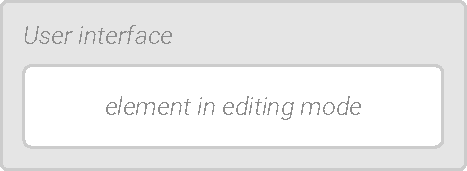
\includegraphics[width=0.5\textwidth]{images/editingmode_usage.pdf}}
%\caption{Usage of HTML editing APIs to implement rich-text editors}
%\label{fig:formatting_dom_tree}
%\end{figure}

\begin{figure}
\centering
%\begin{subfigure}{.5\textwidth}
%  \centering
  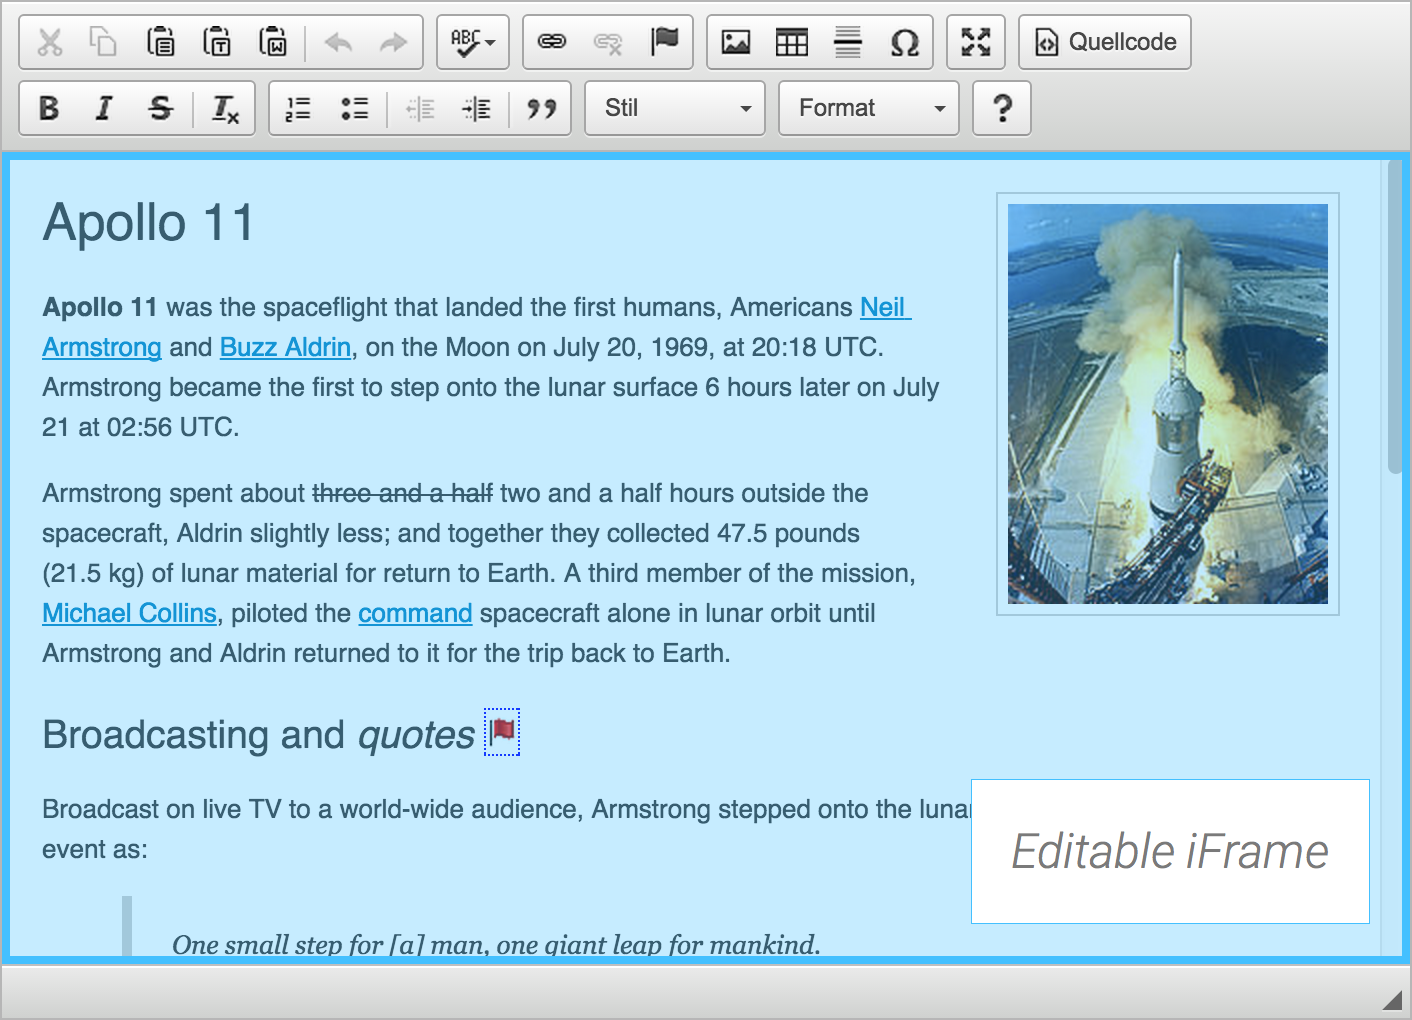
\includegraphics[width=.4\linewidth]{images/ckeditor-demo-overlayed.png}
%  \caption{A subfigure}
%  \label{fig:sub1}
%\end{subfigure}%
%\begin{subfigure}{.5\textwidth}
%  \centering
  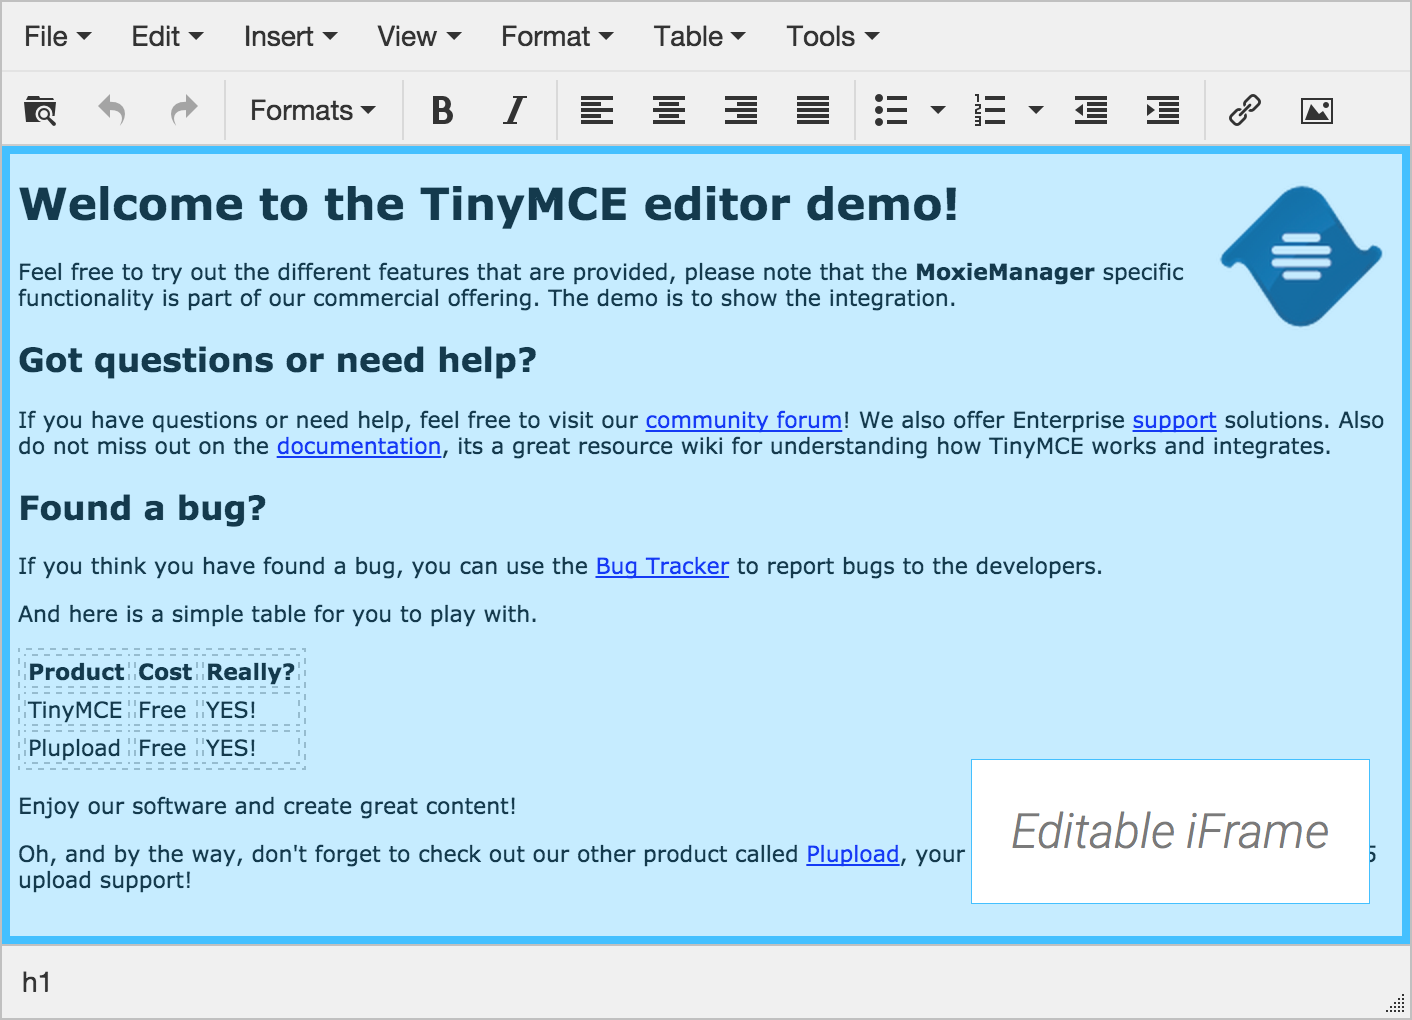
\includegraphics[width=.4\linewidth]{images/tinymce-demo-overlayed.png}
%  \caption{A subfigure}
%  \label{fig:sub2}
%\end{subfigure}
\caption{Usage of HTML editing APIs in CKEditor and TinyMCE}
\label{fig:usage_contenteditable_screenshots}
\end{figure}


Most web-based rich-text editors use HTML editing APIs as their basis. The popular editors ''CKEditor'' and ''TinyMCE'' dynamically create an \texttt{iframe} on instantiation and set its \texttt{body} to editing mode using the \texttt{contenteditable}-attribute. This way, users can type inside the \code{iframe} which acts as a text input field. Both libraries wrap the \texttt{iframe} in a user interface with buttons to format the \texttt{iframe}'s contents. Using the interface, the commands of \texttt{document.execCommand} will be called on the \texttt{iframe}'s \texttt{document} and the selected text will be formatted. While using an \texttt{iframe} is still in practice, many newer editors use a  \texttt{div} element instead. The user interfaces vary between different editors. %Some editors do not show any chrome unless text will be selected

Usually, rich-text editors implemented this way wrap their editing capabilities, including \texttt{document.execCommand}, in an API to enrich functionality and provide higher-level concepts. As discussed in \refpart{part:discussion}, using HTML editing APIs requires a lot of workarounds, which some editors account for in the implementation of their library. Rich-text editing libraries can be downloaded JavaScript files and included in a web project. To display an editor on a website, it is common to select a \code{textarea} element on the website, that the library will replace with the rich-text editor. To integrate the editor into web forms, most libraries will mirror their contents to the selected \code{textarea}, so they can be submitted to a server.

For years, the market of web-based rich-text editors has been dominated by ''CKEditor'' and ''TinyMCE''. Both editors remain among the most popular choices. More recently, the number of editors increased drastically. Popular choices on GitHub, rated by the number of ''stars'', include ''MediumEditor'', ''wysihtml'' and ''Summernote''. As Piotrek Koszuli\'{n}ski points out, most editors ''really doesn't[sic] work''\cite{bj} for the reasons discussed in \refsection{sec:disadvantages_of_html_editing_apis}.

%\textit{Should I elaborate this a bit more?}
